%_____________________________________________________________________________________________
% Chapter 4: System Design
%_____________________________________________________________________________________________

\chapter{System Design}
\label{ch:design}

This chapter describes the design of the final system: its architecture, the benchmark that produces monitored streams with known ground truth, the label-free signals, the two warning tiers, and the protocol used to evaluate them. The history of how the design was reached is given in Chapter~\ref{ch:impl}.

\section{System Architecture}
\figref{fig:arch} shows the architecture as five layers.
\begin{itemize}
\item \textbf{Data.} Public tabular datasets from OpenML feed a benchmark generator, which builds monitored streams with a known intervention batch. Natural row-order streams are used as a reality check.
\item \textbf{Model.} A frozen classifier $f$ is fitted once on a labeled reference set $R$. Each incoming batch $B_t$ is scored by $f$; its labels stay hidden.
\item \textbf{Signals.} Label-free signals are computed per batch: input-shift statistics and model-behaviour statistics.
\item \textbf{Monitor.} Two tiers turn the signals into alerts: a \emph{drift watch} that is sensitive to any drift, and a \emph{harm tier} that estimates whether the drift is lowering accuracy.
\item \textbf{Outputs.} Alerts are confirmed or cleared when delayed labels arrive. Evaluation scripts compute the warning tiers and apply the pre-registered pass rules; the dashboard, paper and this report are generated from the saved results.
\end{itemize}

\begin{figure}[H]
\centering
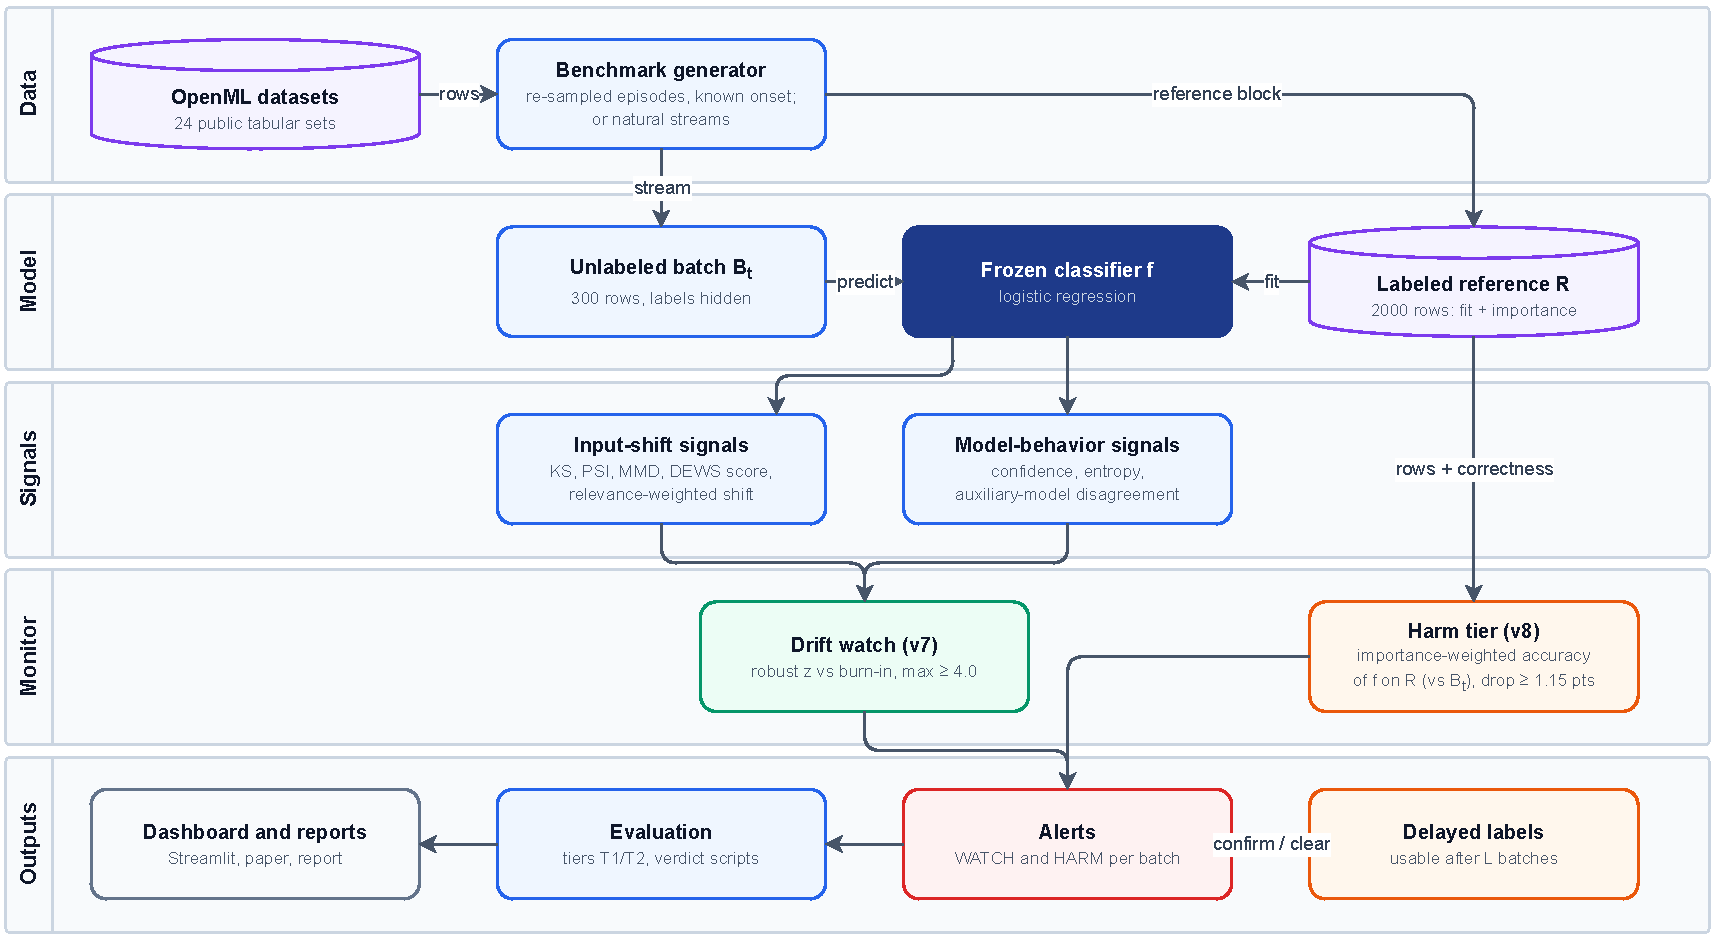
\includegraphics[width=\textwidth]{fig_architecture.pdf}
\caption{Layered architecture of the ML Model Drift Early-Warning System.}
\label{fig:arch}
\end{figure}

\section{Benchmark Design}
\label{sec:benchmark}
Evaluating an early-warning system needs ground truth: we must know when a shift started and whether it actually hurt the model. Synthetic generators provide this but are unrealistic (Section~\ref{sec:v2}); natural streams are realistic but have no known onset. The benchmark combines the two by \emph{re-sampling real rows}.

Each episode draws a contiguous block of a dataset (\figref{fig:episode}):
\begin{itemize}
\item a \textbf{reference} of 2000 rows: $f$ is fitted on the first 1500, and the last 500 are held out to compute $f$'s permutation feature importance;
\item a \textbf{pool} of the next 20,000 rows. Because reference and pool come from the same period, an unshifted stream has no built-in drift.
\end{itemize}
The stream has 45 batches of 300 rows sampled with replacement from the pool; \emph{every row keeps its true label}, so the true accuracy of $f$ on every batch is known. From an onset batch $s \in [10,16]$:
\begin{itemize}
\item \textbf{Gradual or abrupt shift}: rows are sampled with weights proportional to $\exp(\lambda(t)\,\sigma\,z_j)$, where $z_j$ is a standardised feature, $\sigma=\pm 1$ a random direction, and $\lambda$ ramps linearly to 1.5 over 15 batches (gradual) or jumps to 1.5 (abrupt). The feature $j$ is drawn from the more important or the less important half of features with equal probability, so that some shifts are designed to be irrelevant.
\item \textbf{Label change}: labels are flipped with a probability that ramps to 0.3 for rows with $z_k>0$, a change in $P(Y\mid X)$ that input-only signals cannot see.
\item \textbf{Clean}: uniform sampling.
\end{itemize}
Each dataset contributes 10 clean, 30 gradual, 15 abrupt and 10 label-change episodes (65 episodes). Algorithm~\ref{alg:episode} summarises the construction.

\begin{figure}[H]
\centering
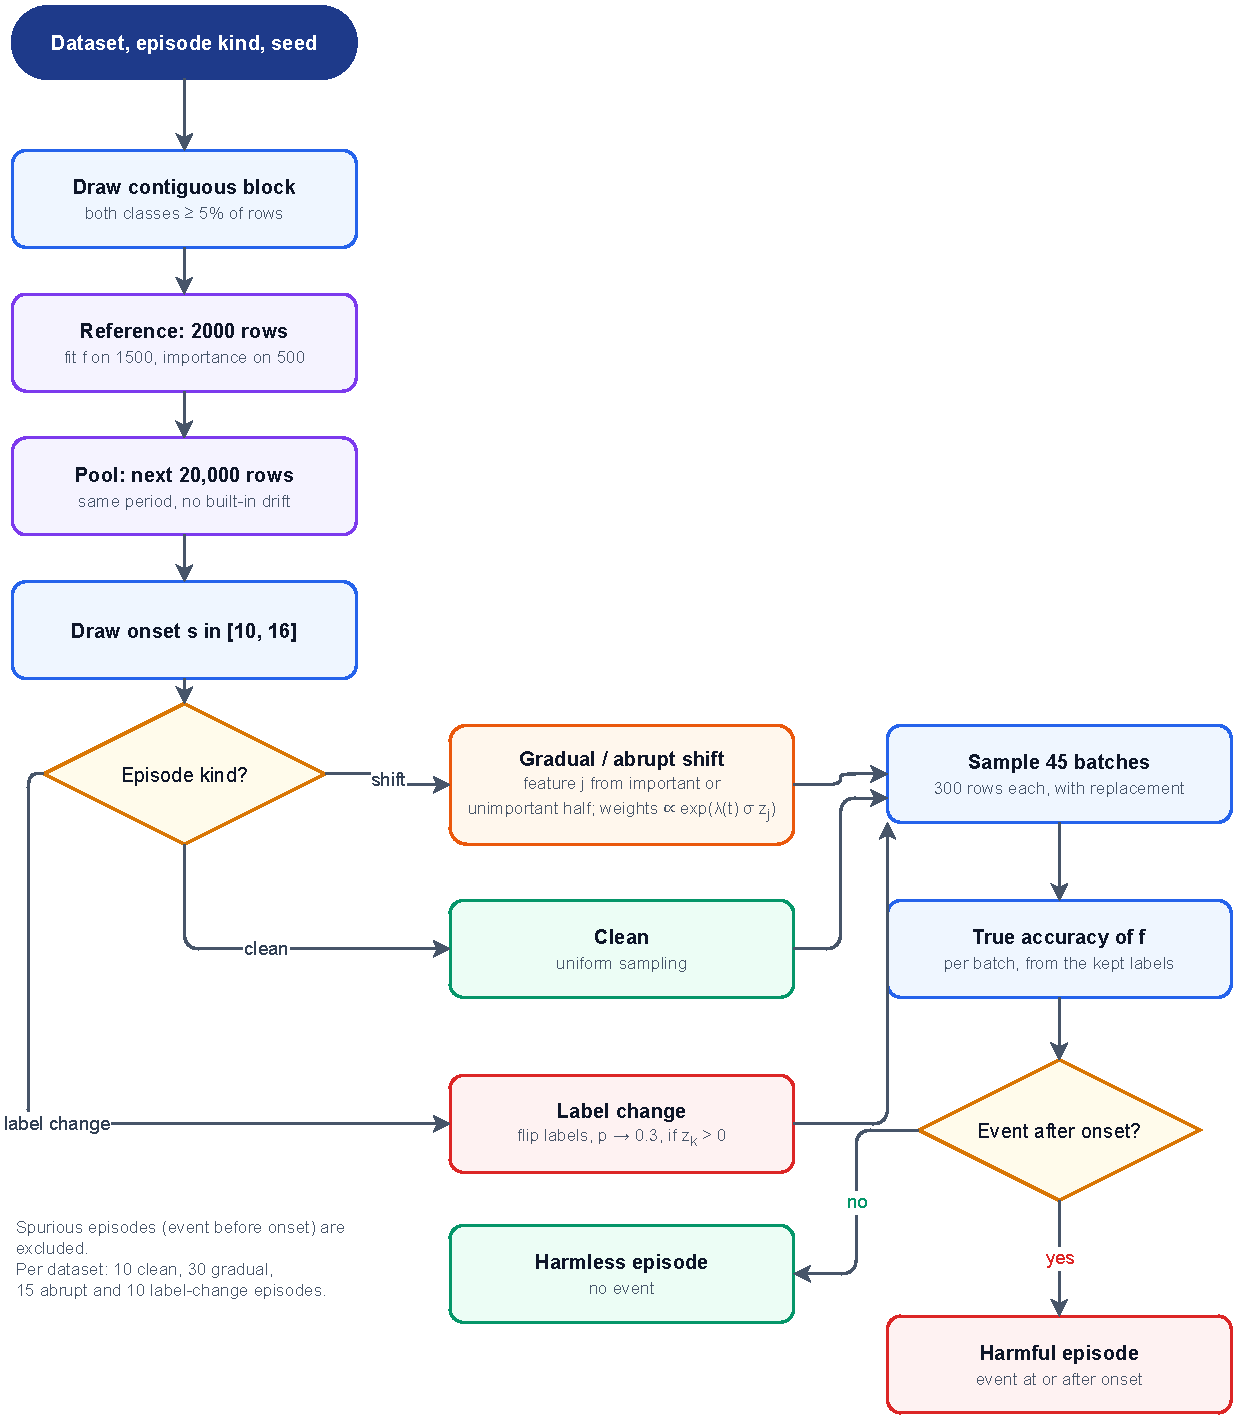
\includegraphics[width=0.82\textwidth]{fig_episode_generation.pdf}
\caption{Flowchart of benchmark episode generation.}
\label{fig:episode}
\end{figure}

\begin{algorithm}[H]
\caption{Building one benchmark episode}
\label{alg:episode}
\begin{algorithmic}[1]
\Require dataset $(X, y)$, episode kind, seed
\State draw a block start where both classes are $\geq$5\% of the fit rows and of the pool
\State $R \gets$ next 2000 rows; fit $f$ on the first 1500; permutation importance on the last 500
\State $P \gets$ next 20{,}000 rows (pool); draw onset $s \in [10,16]$
\If{kind is a shift} \State pick feature $j$ (important or unimportant half) and sign $\sigma$ \EndIf
\For{$t = 0, \dots, 44$}
  \If{kind is a shift and $t \geq s$}
    \State sample 300 rows of $P$ with weights $\propto \exp(\lambda(t)\,\sigma\, z_j)$
  \Else
    \State sample 300 rows of $P$ uniformly
  \EndIf
  \If{kind is a label change and $t \geq s$} \State flip labels of rows with $z_k > 0$ with probability $0.3\,\min(1, (t-s+1)/15)$ \EndIf
\EndFor
\State compute the accuracy of $f$ on every batch; label the episode harmful, harmless, clean or spurious
\end{algorithmic}
\end{algorithm}

\subsection{Datasets and data groups}
All datasets are binary (or reduced to majority class versus the rest) and use their first 20 non-constant features. \tabref{tab:groups} shows how they were used. The 13 v6 datasets had already been used as natural-order streams in the exploratory studies v1--v5; the confirmation groups of v7, v8 and v10 were downloaded only after the corresponding design was frozen and had never been used before. The full list is in Appendix~\ref{app:data}.

\begin{table}[H]
\caption{Data groups and their use (65 episodes per dataset).}
\label{tab:groups}
\centering
\small
\begin{tabular}{@{}lcl@{}}
\toprule
Group & Datasets & Use \\
\midrule
v6 development & 8 & design, thresholds and all later tuning \\
v6 held-out & 5 & one-time v6 verdict (seen in v1--v5 as natural streams) \\
v7 confirmation & 6 & one-time drift-watch verdict \\
v8 confirmation & 5 & one-time harm-tier verdict \\
v10 confirmation & 6 & one-time test of stricter alerting rules \\
Natural streams & 13 & 328 row-order windows, no injected shift (H5, C5) \\
\bottomrule
\end{tabular}
\end{table}

\section{Label-Free Signals}
\tabref{tab:signals_def} lists the signals computed for every batch without labels. They fall into two families. \emph{Input-shift} signals compare the batch's inputs with the reference; \emph{model-behaviour} signals describe how the model reacts to the batch.

\begin{table}[H]
\caption{Label-free signals computed per batch.}
\label{tab:signals_def}
\centering
\small
\begin{tabularx}{\textwidth}{@{}p{3.6cm}p{2.3cm}X@{}}
\toprule
Signal & Family & Definition \\
\midrule
Fused DEWS drift score & input shift & original prototype's weighted fusion of per-feature KS/PSI statistics, embedding MMD and a confidence component \\
Mean KS & input shift & mean two-sample KS statistic over features \\
Relevance-weighted shift & input shift & $\sum_j \text{importance}_j \cdot \mathrm{KS}_j$, using $f$'s permutation importance \\
Positive-rate shift & input shift & absolute change of the share of positive predictions from its burn-in mean \\
Confidence drop & behaviour & negative mean top-class probability of $f$ \\
Entropy & behaviour & mean prediction entropy of $f$ \\
Disagreement & behaviour & share of rows where $f$ disagrees with a random forest~\cite{breiman2001rf} and a gradient-boosting model~\cite{friedman2001gbm} trained on the same reference rows \\
\bottomrule
\end{tabularx}
\end{table}

\section{The Two-Tier Monitor}
\label{sec:twotier}
\figref{fig:twotier} shows how one batch flows through both tiers and how delayed labels later confirm or clear an alert.

\begin{figure}[H]
\centering
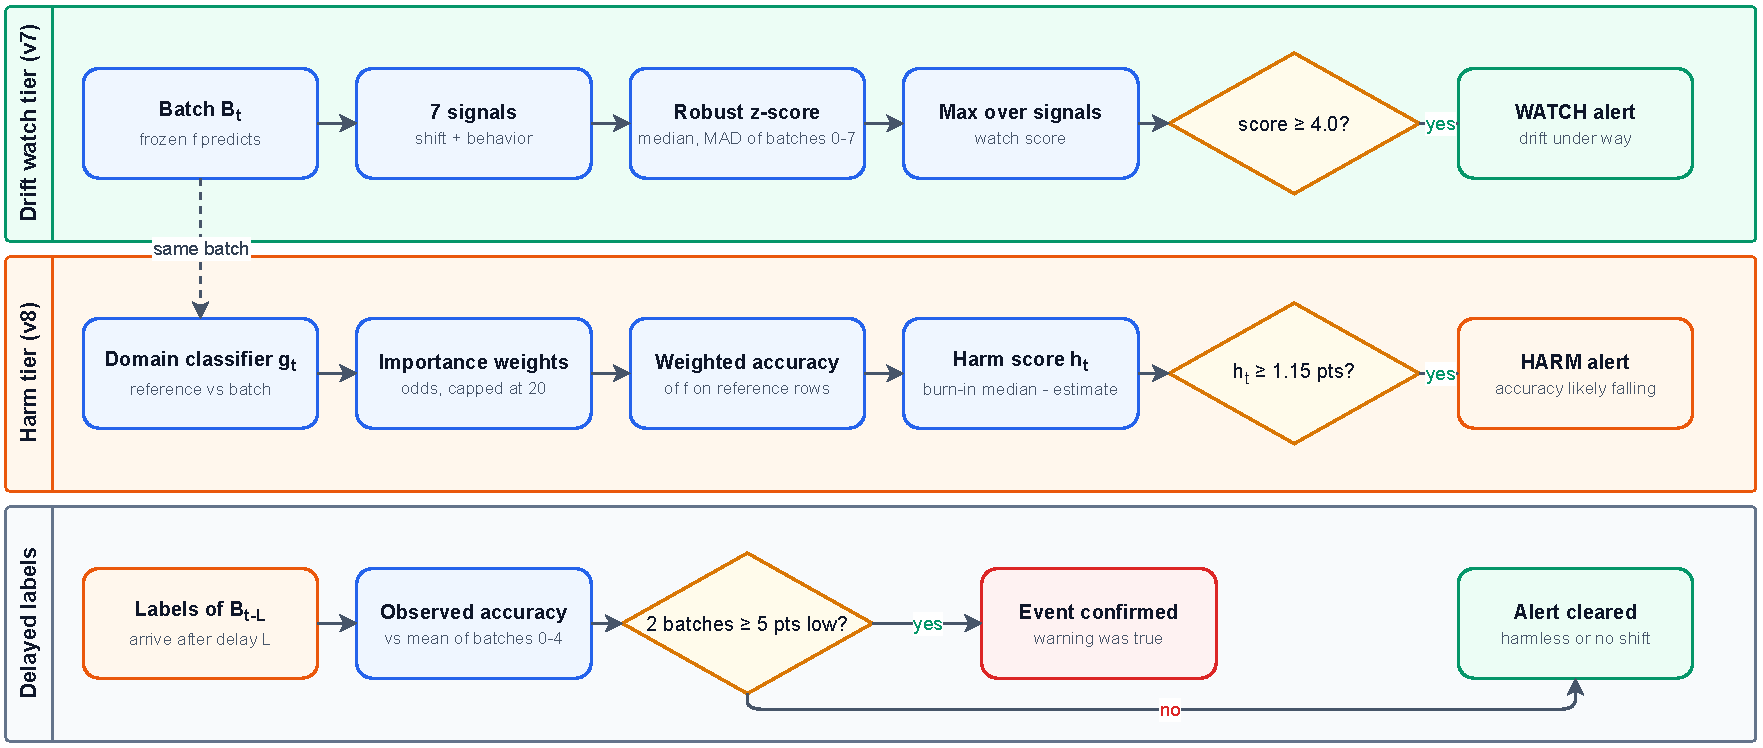
\includegraphics[width=\textwidth]{fig_two_tier_flow.pdf}
\caption{Per-batch data flow of the two-tier monitor and the confirmation by delayed labels.}
\label{fig:twotier}
\end{figure}

\subsection{Tier 1: drift watch (v7)}
Raw drift statistics live in dataset-specific units: a KS statistic of 0.1 may be normal noise on one dataset and a large shift on another. The drift watch therefore expresses every signal relative to the stream's own burn-in. For a signal $x_t$,
\begin{equation}
z_t = \frac{x_t - \mathrm{med}(x_{0:8})}{\max\left(1.4826\,\mathrm{MAD}(x_{0:8}),\ 0.01\right)},
\end{equation}
a robust z-score in which the median and the median absolute deviation (scaled to match a standard deviation for normal data) are computed on batches 0--7. The drift-watch score is the maximum $z_t$ over the seven signals of \tabref{tab:signals_def}. A WATCH alert is raised when the score exceeds \textbf{4.011} standard deviations, a threshold chosen on development data. Because the score is measured in deviations from the stream's own normal, the same threshold is comparable across streams that start in a stable period.

\subsection{Tier 2: harm tier (v8)}
\label{sec:harm}
Whether a shift harms the model depends on whether it moves the data into regions where this particular model is wrong. The labeled reference set shows where that is. For each batch $B_t$, a logistic domain classifier $g_t$ is trained to separate reference rows (label 0) from batch rows (label 1). For reference row $x_i$ with correctness $c_i = \mathbb{1}[f(x_i)=y_i]$, the importance weight and the label-free accuracy estimate are
\begin{equation}
w_i = \min\!\left(\frac{\rho_i}{\bar\rho},\ 20\right),\quad \rho_i=\frac{g_t(x_i)}{1-g_t(x_i)},\qquad \hat a_t = \frac{\sum_i w_i c_i}{\sum_i w_i},
\label{eq:iw}
\end{equation}
where $\bar\rho$ is the mean odds over the reference. Under covariate shift, $\hat a_t$ targets the accuracy of $f$ on $B_t$~\cite{shimodaira2000,sugiyama2007iwcv}. The harm score is the estimated drop since the burn-in,
\begin{equation}
h_t = \mathrm{med}(\hat a_{0:8}) - \hat a_t,
\end{equation}
in accuracy units. A HARM alert is raised when $h_t \ge 0.0115$ (an estimated drop of 1.15 accuracy points). The harm tier has no trained parameters beyond this threshold. Pure label changes are invisible to it by construction.

\subsection{Threshold selection}
Thresholds are chosen on development data only, with false alerts kept within 5 per 100 clean batches:
\begin{itemize}
\item \textbf{v6 rule} (also used by the drift watch): the threshold with the highest development T1 share; ties go to the higher threshold.
\item \textbf{Separation rule} (harm tier): the threshold that maximises the T2 share on harmful shifts minus the alert share on harmless shifts.
\end{itemize}

\section{Evaluation Protocol and Pre-Registration}
\label{sec:prereg}
Every experiment from v6 onward followed the workflow of \figref{fig:prereg}. Before any confirmation data were obtained, a configuration module defining the datasets, seeds, method, threshold rule and each hypothesis with its pass rule was committed to git. Thresholds were chosen on development data and frozen in JSON files whose SHA-256 fingerprints were recorded in the protocol; the confirmation script refuses to run if a fingerprint does not match. Deviations, for example shuffling a dataset whose rows are stored sorted by class, were logged with date and reason before any affected episode was built. Each verdict was then computed once, by a script that applies the frozen pass rules.

\begin{figure}[H]
\centering
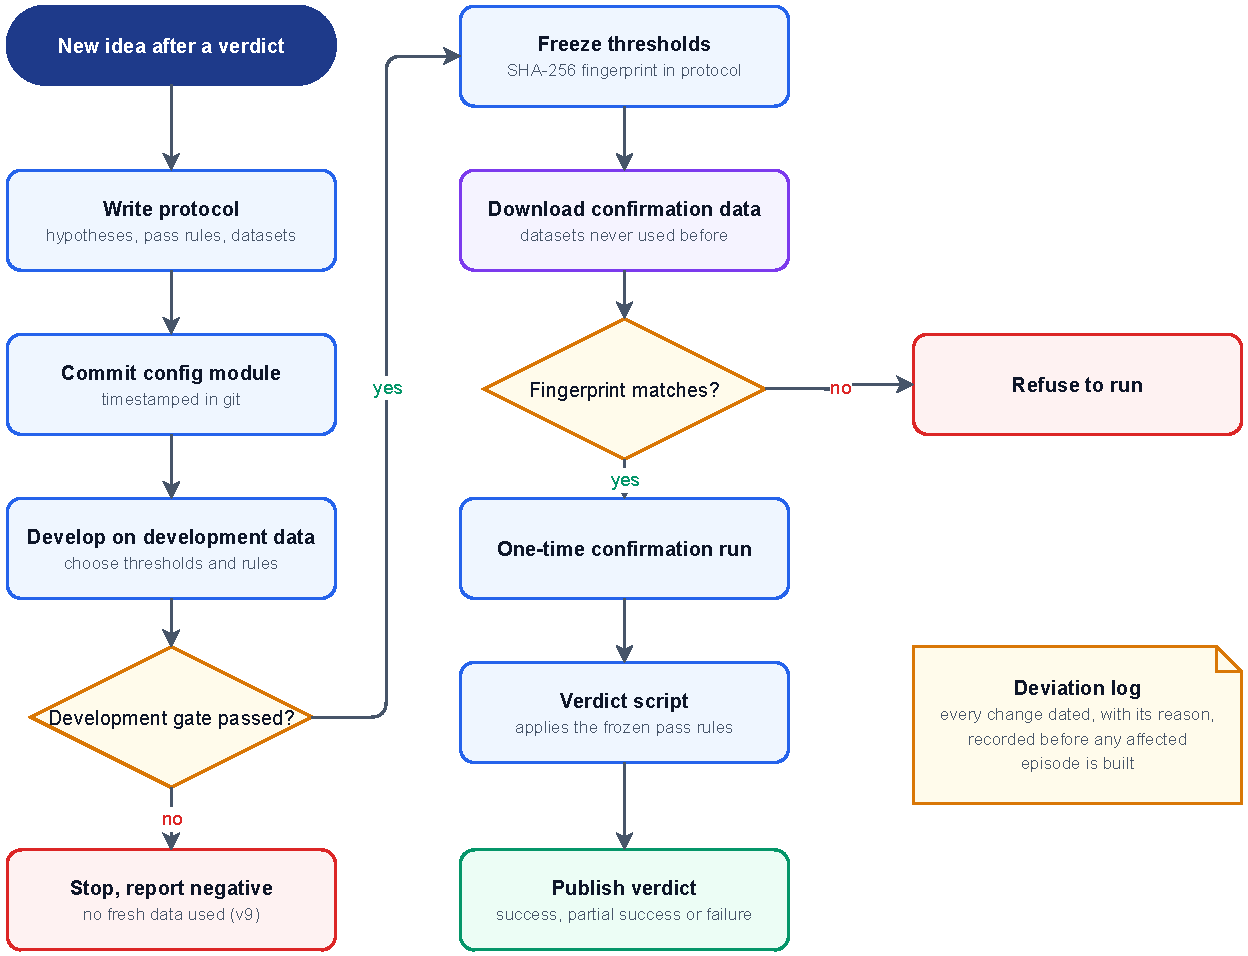
\includegraphics[width=0.92\textwidth]{fig_preregistration.pdf}
\caption{Pre-registration workflow used for every experiment from v6 onward.}
\label{fig:prereg}
\end{figure}

Confidence intervals are 95\% bootstrap intervals over episodes with 2000 resamples~\cite{efron1979bootstrap}; comparisons between two methods use a paired bootstrap that resamples the same episodes for both.

\section{Software Design}
\figref{fig:modules} shows the main parts of the code base and how they depend on each other. The core library \texttt{dews/} contains the benchmark, signal extraction, evaluation metrics, monitors and harm estimation. Experiment runners in \texttt{scripts/} use the library, read the frozen configurations and write all outputs to \texttt{artifacts/}. The dashboard, the paper figures and this report read only from \texttt{artifacts/}, so every number shown can be traced back to a saved result.

\begin{figure}[H]
\centering
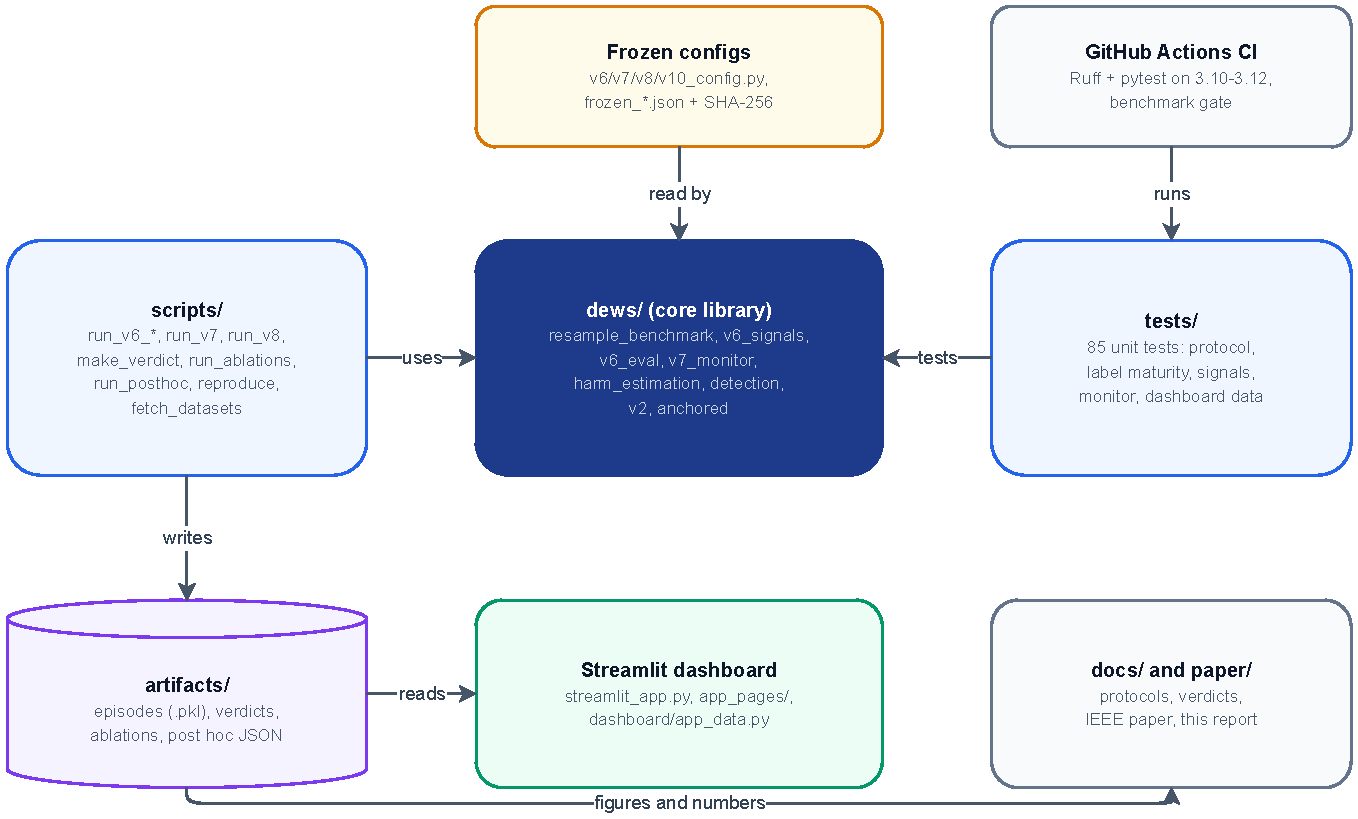
\includegraphics[width=0.9\textwidth]{fig_modules.pdf}
\caption{Software modules and their dependencies.}
\label{fig:modules}
\end{figure}

\subsection{Dashboard design}
The dashboard (\figref{fig:dashflow}) is a Streamlit~\cite{streamlit} application with four pages. A plain Python module, \texttt{dashboard/app\_data.py}, contains all data loading and replay logic without any Streamlit imports, so that it can be unit-tested. The \emph{replay} function reproduces exactly what the monitor knew at each batch: labels appear only after the selected delay, and scores are compared with the frozen thresholds.

\begin{figure}[H]
\centering
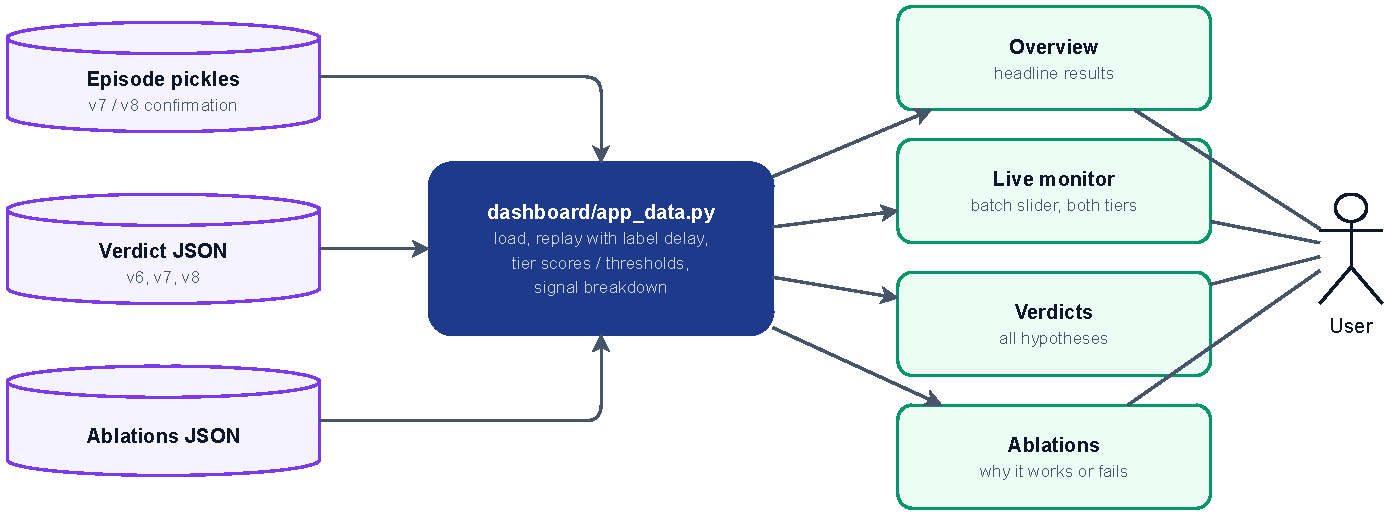
\includegraphics[width=0.95\textwidth]{fig_dashboard_flow.pdf}
\caption{Data flow of the Streamlit dashboard.}
\label{fig:dashflow}
\end{figure}
